\chaptr{Anexos}{anexos}
\sect{Anexo A: Tareas del desarrollo}{anexoA}

Durante todo el desarrollo del proyecto se han realizado una serie de tareas, para las cuales se ha utilizado la
herramienta
\boldFont{Notion}.\ Esta herramienta proporciona una interfaz muy sencilla para la creación de listas de tareas, con la
posibilidad de añadir etiquetas, asignar responsables, añadir comentarios, entre otras funcionalidades.\ A continuación
se incluye el fichero pdf generado por Notion con las tareas realizadas durante el desarrollo del proyecto.
%El proyecto completo se puede consultar en el siguiente enlace:
%\url{https://scastd00.notion.site/9c59c2812d8b440faa453924fef2f320?v=20f7c2f47dd64574ac57713e8efe2718}.

% Todo: include this pdf
\label{anx:product-backlog-notion}
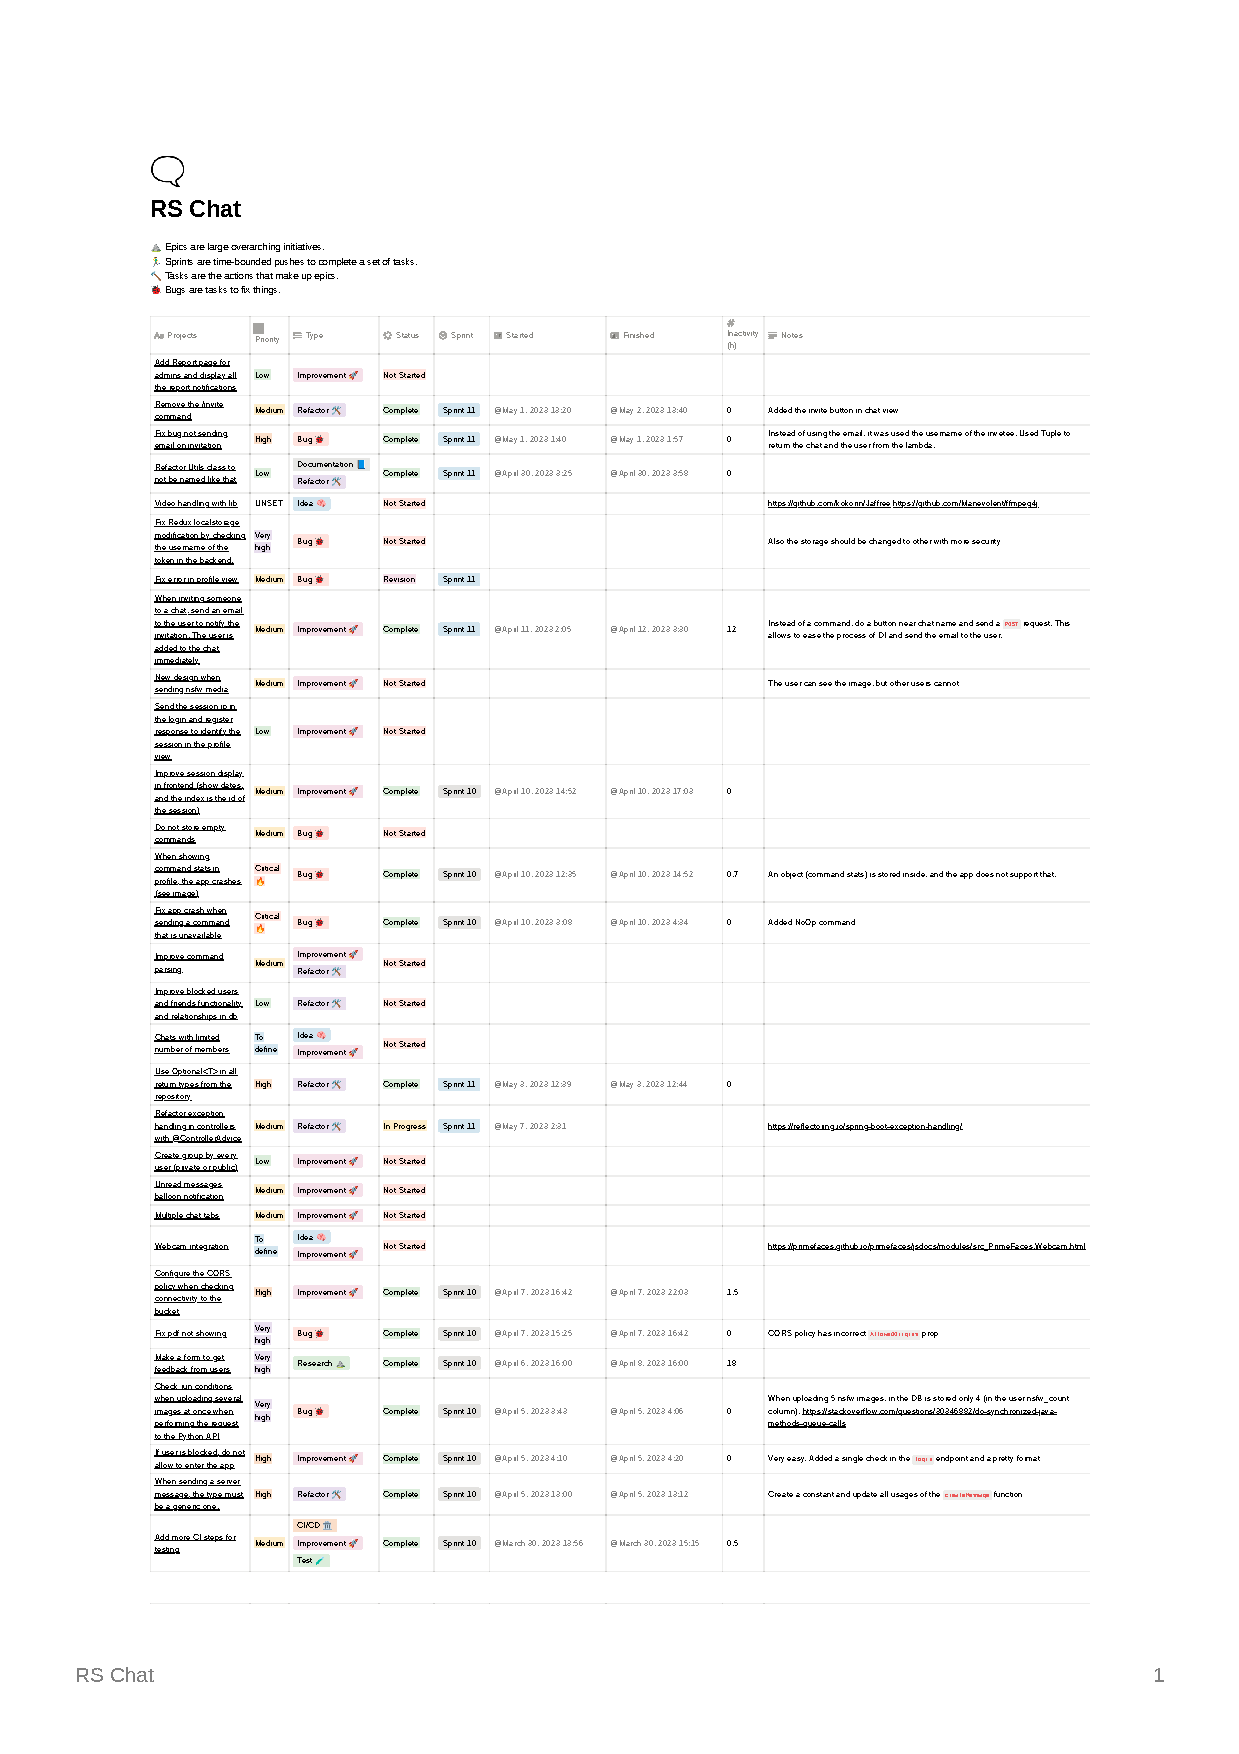
\includepdf[pages=-]{anexos/TareasNotion.pdf}
